\documentclass[12pt]{notes}



% For SAS Code
\usepackage{listings}
\usepackage{hyperref}

\usepackage{wrapfig}

% In order for the minted code to run, we had to create a new compilation routine called pdflatex+shellEscape.
% This includes a --shell-escape command which should ONLY be used when pygmentized is required as it compromises security. 
% We also had to add pygmentize (a python package) to the system path (BEFORE miktex) and then restart the computer. 
\usepackage{minted}
\usemintedstyle{borland}
\lstset{language=SAS, 
  breaklines=true,  
  basicstyle=\ttfamily\bfseries,
  columns=fixed,
  keepspaces=true,
  identifierstyle=\color{blue}\ttfamily,
  keywordstyle=\color{cyan}\ttfamily,
  stringstyle=\color{purple}\ttfamily,
  commentstyle=\color{green}\ttfamily,
  } 
  
% Command for Questions
%\question{}

% Command for Notes
% \note{}

% Code to create a minipage where you can type in class notes. 
%%\begin{minipage}[l][2cm][c]{\textwidth}
\begin{comment}

\end{comment}
%%\end{minipage}


% Begin Document
%==============================================================================
\begin{document}
% Include the Title of the Handout
\ntitle{1.3: SAS Crash Course}

% Include Numbered Sections
\section{Why SAS?}

SAS is a popular statistical software package used by many companies in researchers. 

\nspace
Advantages:
\begin{itemize}
\item Lots of output without having to write much code. 
\item Provides lots of graphical diagnostics automatically. 
\end{itemize}

\nspace
Disadvantages: 
\begin{itemize}
\item Expensive (if you want a desktop version).
\item Hard to customize output (particularly visualizations). 
\end{itemize}

\nspace
Teaching SAS in this class:
\begin{itemize}
\item (For non-math majors): Has the smallest learning curve to create basic linear models. 
\item (For math and stats students): Provides you exposure to multiple programming languages as several of our upper division courses use R.
\end{itemize}

In this class, we will focus on using SAS Studio, which is a free online version of SAS. 

\section{SAS Studio Online}
% You can mention that there are several computers on Campus that have a desktop version of SAS installed on them.
% Students may choose to simply do their homework and projects in this lab. 
\begin{itemize}
\item Navigate to \url{https://odamid.oda.sas.com/SASLogon/login?service=https%3A%2F%2Fodamid.oda.sas.com%2FSASODAControlCenter%2Fj_spring_cas_security_check}.
\item Select the ``Not registered or cannot sign in?'' option. 
\item Follow directions for creating a SAS profile. 
\item Note that the email confirming your profile may take some time (5-10 minutes) to receive.
\item Note also that the only tool we will use in this class is ``SAS Studio''.
\end{itemize}

\section{Getting Started}
Once you have an account, your SAS studio window will look something like this. 
\begin{figure}[H]
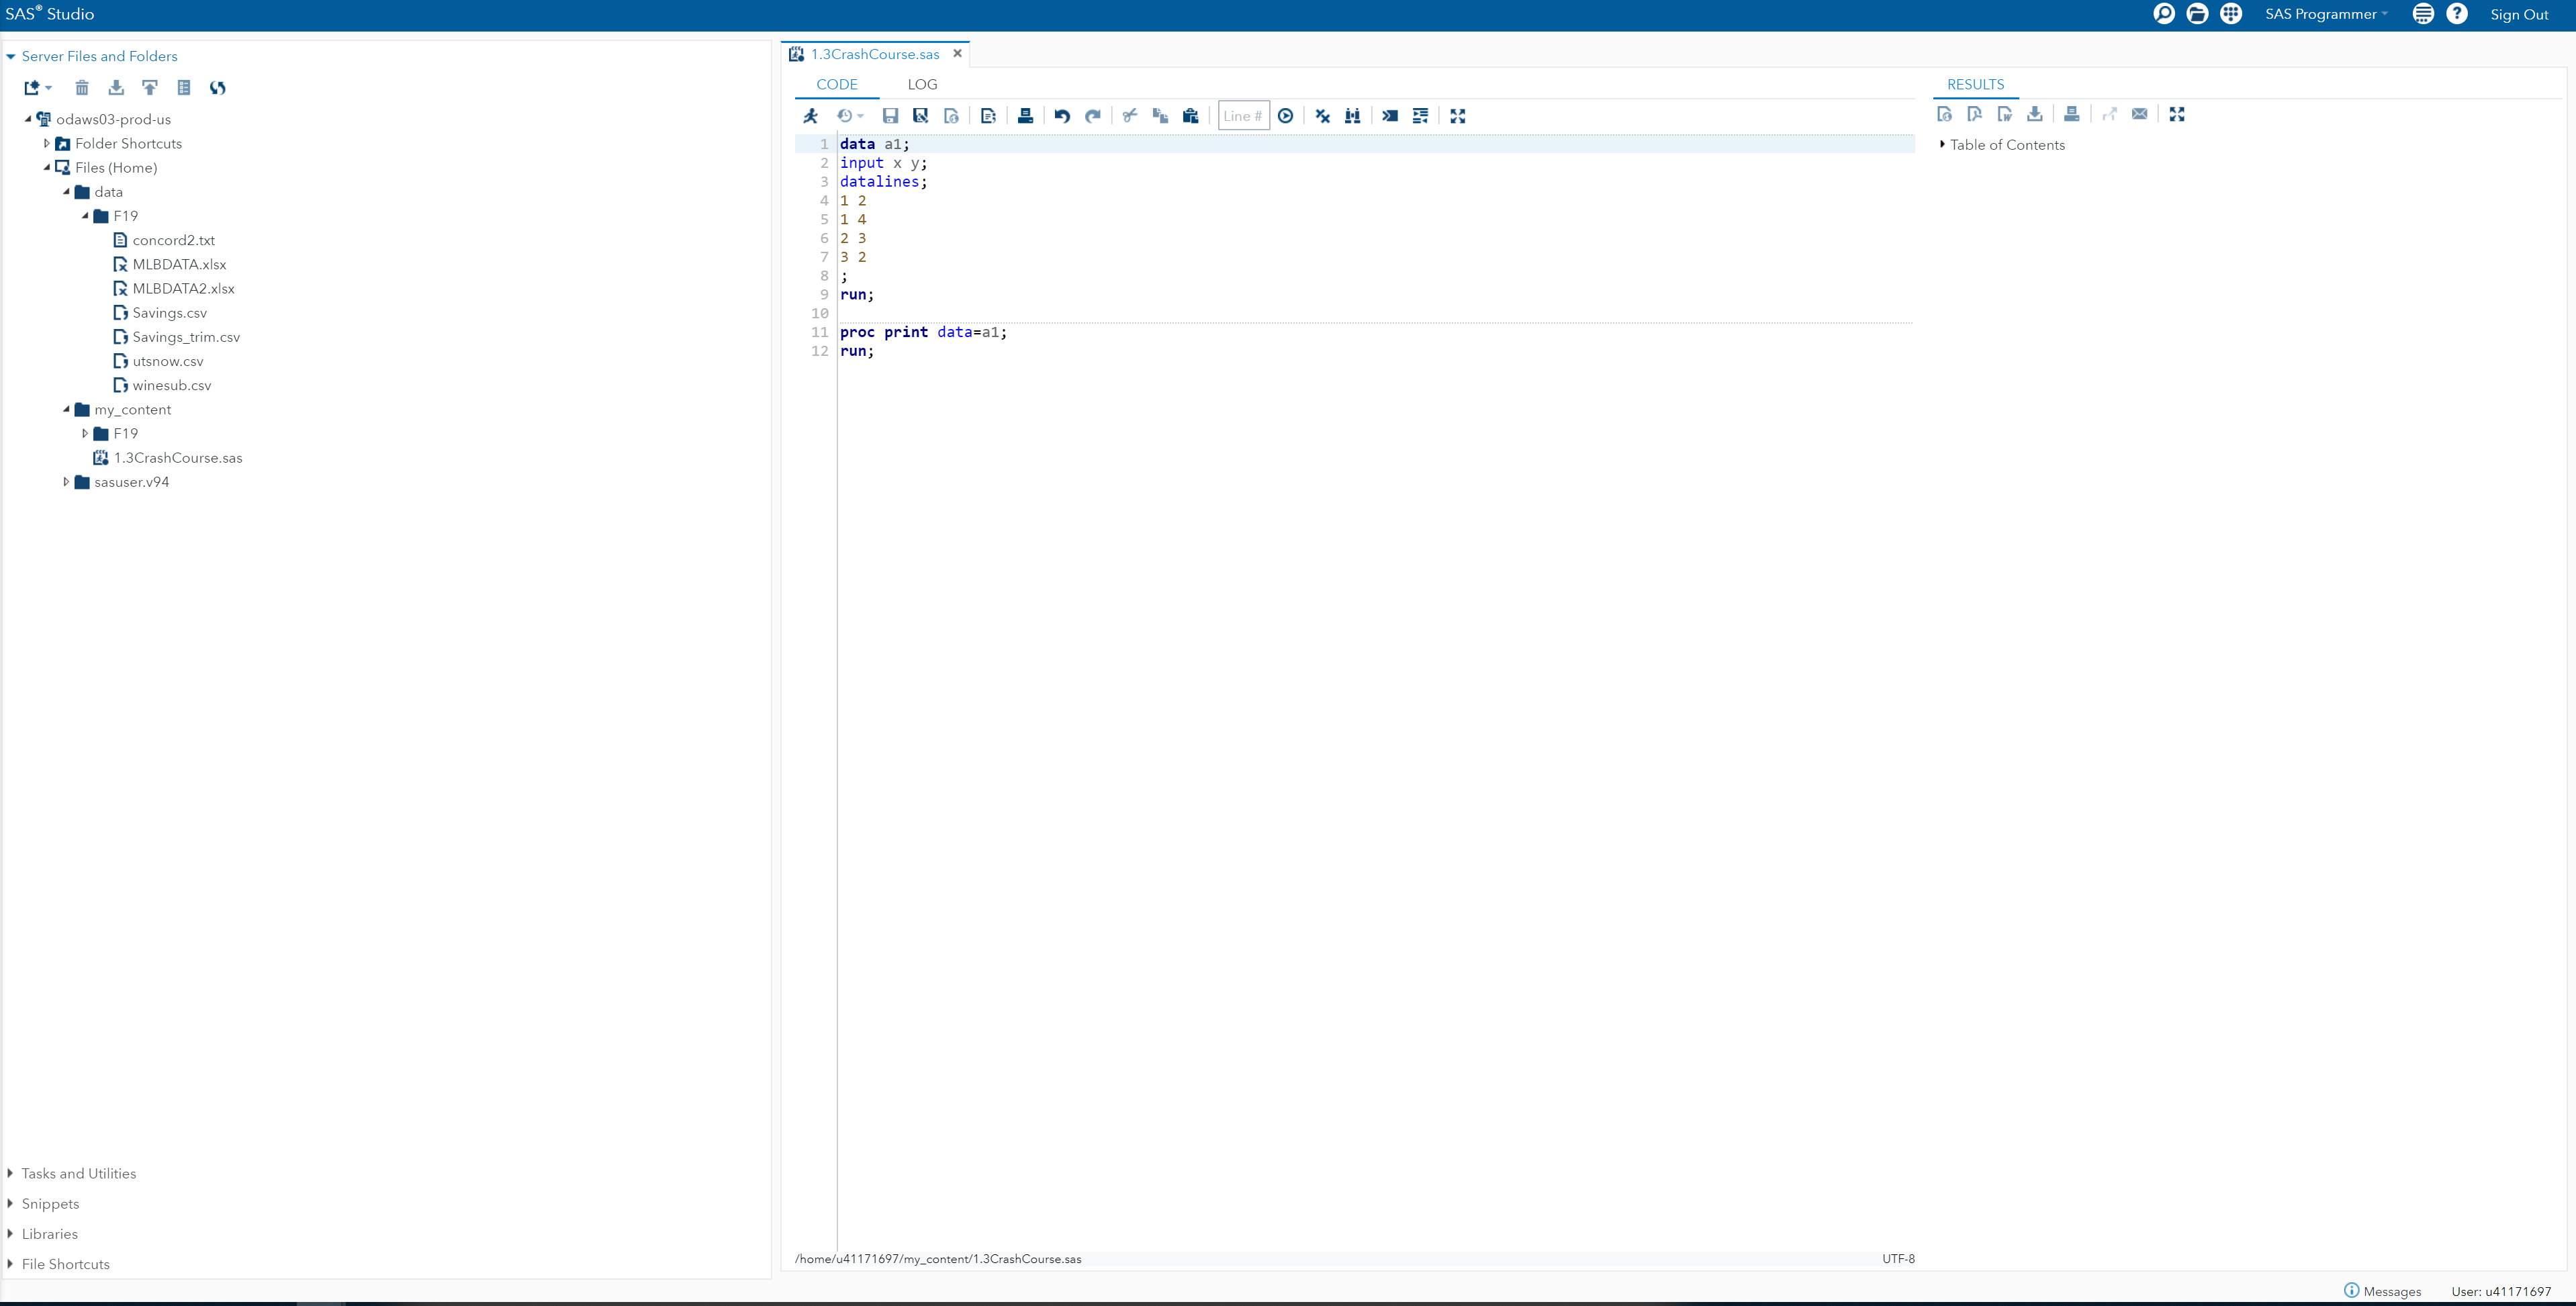
\includegraphics[width = \textwidth]{figures/module1/SASstudio.png}
\caption{Sample SAS studio interface.}
\end{figure}

\nspace
Main windows:
\begin{itemize}
\item CODE (or Editor): The window where you type in SAS commands. Font color matters in this window. 
\item LOG: tells what was ``done''. Red notes indicate errors. This is the first thing you should check if your results are unexpected. 
\item RESULTS (or Results Viewer): displays results in HTML format. You can export the HTML output as a pdf or a rft (rich text file - Microsoft word) to obtain nice looking output that you can copy into your reports. Or, you can use the snipping tool to save relevant output and import them as figures in LaTeX (more on LaTeX in 1.4). 
\end{itemize}


You run SAS code by clicking on the ``Running Man''. 


\begin{figure}[H]
\centering

\includegraphics{figures/module1/runningman.png}
\end{figure}

\nspace
\textbf{Necessary Components of a SAS Program:}
\begin{itemize}
\item a semi-colon at the end of every statement 
\item a data statement that either creates or imports a dataset
\item at least one space between each word or statement
\item (almost always) a \textbf{procedure} that performs some type of analysis with your data
\item a run statement 
\end{itemize}

\subsection*{Data}
There are three ways to read data into SAS. The first way is the easiest, but also not practical for large datasets. 

\subsubsection*{Read in data ``by hand''}
\begin{minted}{sas}
/* Text between the asterisks are considered comments in SAS */

data a1; /* Create a new dataset named a1 */
input x y; /* List the variable names of the data that will be included in a1 */
datalines;  /* (or 'cards') tells SAS to start reading in data */
1 2
1 4
2 3
3 2
;
run; /* Tells SAS to execute the above code */

proc print data = a2; /* Print the dataset to the output screen */
run;
\end{minted}

\begin{figure}[H]
\centering
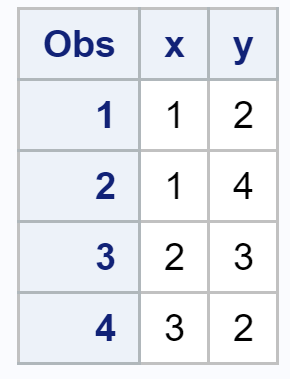
\includegraphics[width = 0.2\textwidth]{figures/module1/sas1.png}
\end{figure}

\subsubsection*{Read in data from a file.}
Assume that the same data as before our located in the SAS studio folder:
\begin{center}
\texttt{/home/u41171697/data/mydata.txt}
\end{center}

\nspace
\textit{Note that SAS Studio will not recognize file paths on your actual computer.} All data that you wish to read into SAS must be uploaded to SAS studio first. 

\nspace
We could read the data directly from the file using:

\begin{minted}{sas}
data a1; 
infile '/home/u41171697/data/mydata.txt'; /* Specify path to file */
input x y; 
run; 
\end{minted}

\subsubsection*{Read in data from a file using a procedure.}
Now suppose that the data are in the excel file mydata.xlsx with the variable names included on the first row. 

\begin{minted}{sas}
proc import
datafile =  ''/home/u41171697/data/mydata.txt'' 
dbms=xlsx /* Specify the file type (what separates the variables) */
out=work.a1 /* Specify the name of the dataset */
replace; /* Overwrite any datasets in the directory with the same name */
run; 
\end{minted}

\subsubsection*{Altering Datasets}
We can add or change variables in a dataset using the commands:

\begin{minted}{sas}
data a2; 
set a1; /* Create a copy of the dataset a1 */
  xy = x*y; /* Multiplication */
  xsq = x**2; /* Exponentiation */
  xeq1 = 0;
  if x = 1 then xeq1=1; /* Conditional Assignment */
run;

proc print data = a2; 
var x y xy xeq1; /* Print all variables to the screen except xsq */
run;
\end{minted}

\begin{figure}[H]
\centering
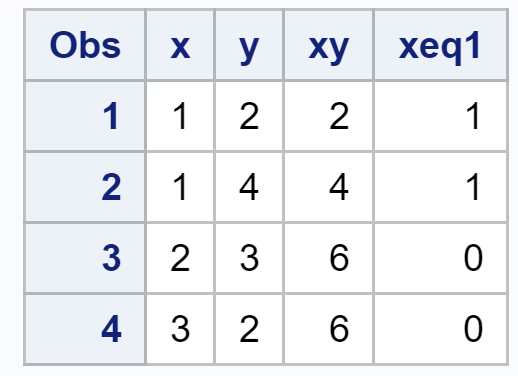
\includegraphics[width = 0.3\textwidth]{figures/module1/sas2.png}
\end{figure}

\subsubsection*{Filtering Datasets}
We can subset datasets using conditional statements.

\begin{minted}{sas}
data a3; set a2;
  if y < 3.5;
    /* Default 'then' is keep */
run;
/* Same as: */
data a3; set a2;
  if y >= 3.5 then delete;
run;
proc print data=a3;
 var x y xeq1;
 title1 'Smaller Set';
run;
\end{minted}

\begin{figure}[H]
\centering
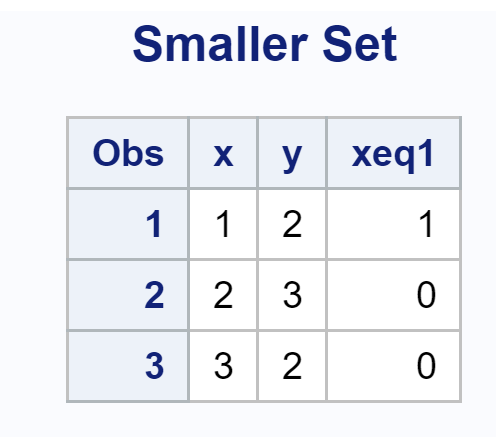
\includegraphics[width = 0.3\textwidth]{figures/module1/sas3.png}
\end{figure}

\subsection*{Procedures}
We prepare data in a SAS-friendly format using DATA steps. We analyze data using SAS procedures (PROC). Some PROCs that we will commonly use in this class include:
\begin{itemize}
\item Fitting models: PROC REG, PROC LOGISTIC, PROC ARIMA, and more
\item Graphical Checks: PROC SGPLOT, PROC SGSCATTER, PROC BOXPLOT, PROC UNIVARIATE
\end{itemize} 

\begin{minted}{sas}
proc sgplot data=a2;
  scatter x=x y=y ;
  title1 'A Simple Scatter Plot';
run;
\end{minted}


\begin{figure}[H]
\centering
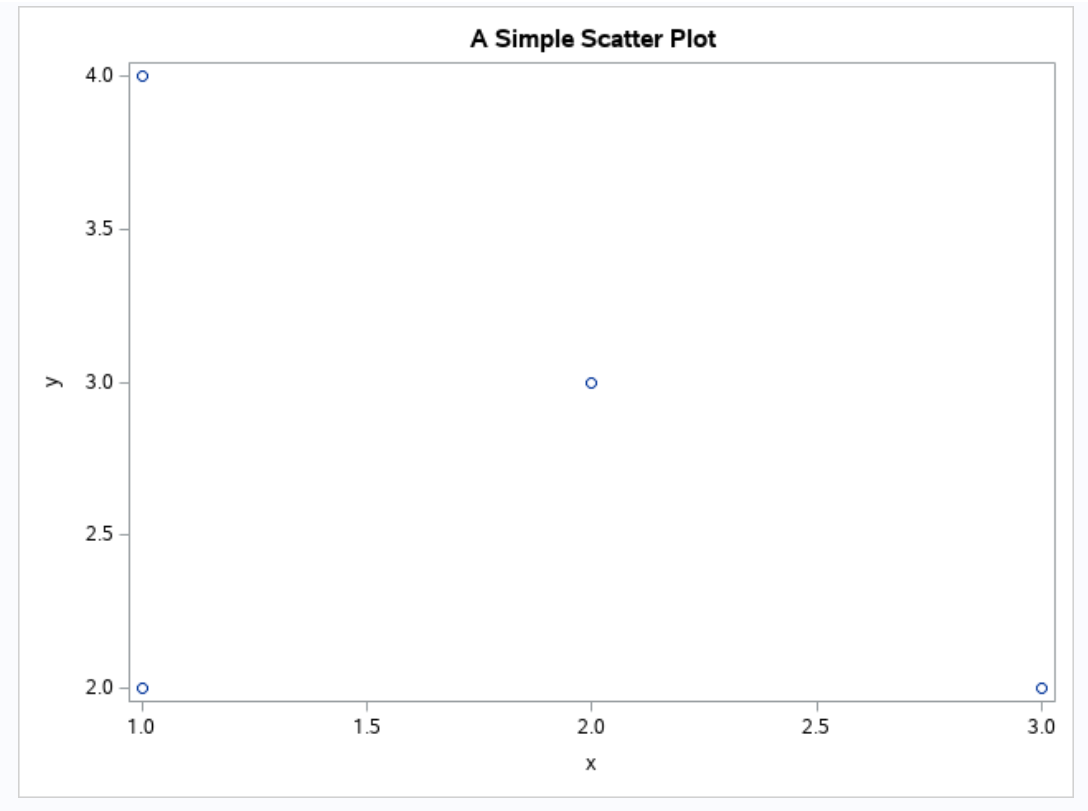
\includegraphics[width = 0.4\textwidth]{figures/module1/sas4.png}
\end{figure}

\begin{minted}{sas}
proc sgplot data=a2;
  scatter x=x y=y /
    markerattrs=(symbol='CIRCLEFILLED'
                 size=12);
  xaxis min=.5 max=3.5 grid
    label='Name of X';
  yaxis values=(1 to 5 by 1) 
    label='Y Name Here'
    labelattrs=(size=20 style=ITALIC);
  title1 height=2 color=grey 
    'A Modified Scatter Plot';
run;
\end{minted}

\begin{figure}[H]
\centering
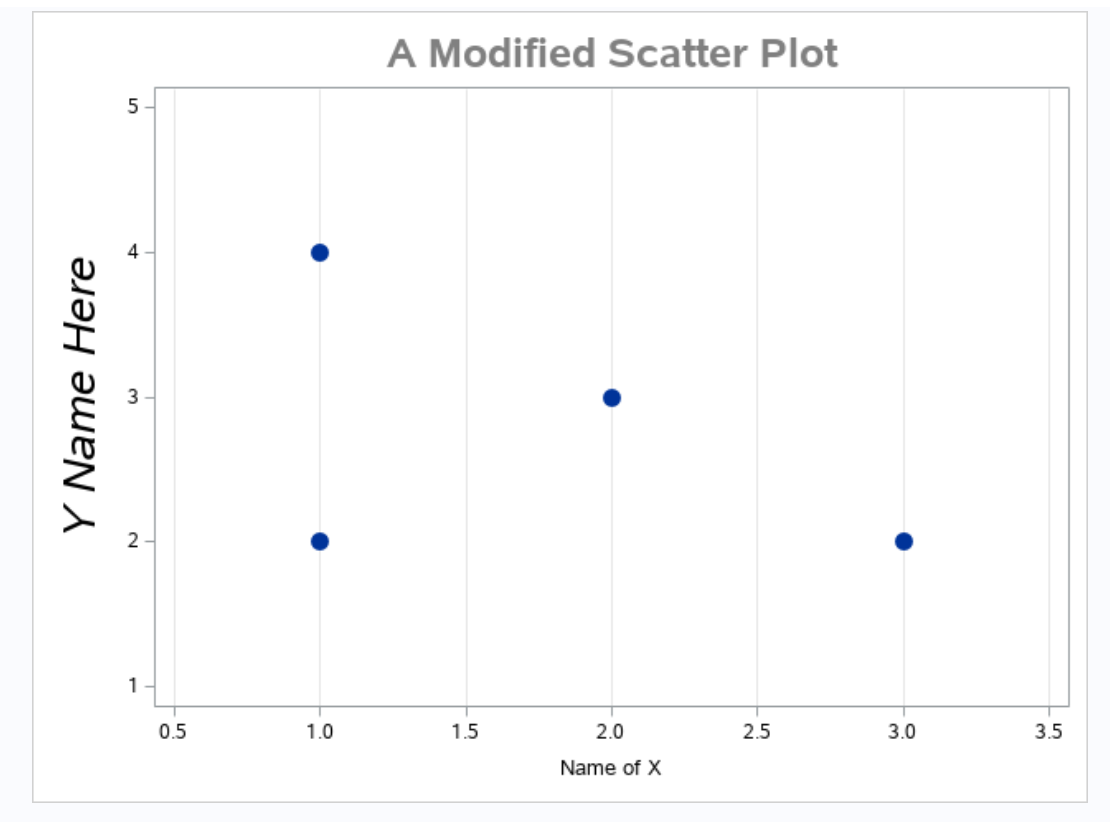
\includegraphics[width = 0.45\textwidth]{figures/module1/sas5.png}
\end{figure}

\begin{minted}{sas}
/ * @@ reads symbols in variable order and ignores new lines
$ indicates that variable z is a character and not numeric 
. - indicates missing values */
 data a1; input x y z $ @@; cards;
   1 2 alpha   1 4 .
   2 3 gamma   3 . delta
   ;
 run;
 proc means data=a1;
   var y;
   title1 "Means Output";
 run;
 proc print data=a1;
   var y x z;
   title2 "Subtitle";
run;
\end{minted}

\begin{figure}[H]
\centering
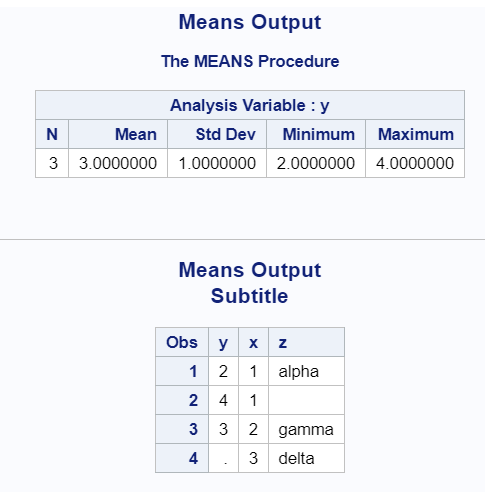
\includegraphics[width = 0.45\textwidth]{figures/module1/sas6.png}
\end{figure}

\section{Miscellaneous Notes}
\begin{itemize}
\item Missing semicolons are perhaps the most common bug in SAS code. 
\item The best way to get started with SAS programming is to look at the course example code, then figure out how to modify that code for your particular problem. 
\item Export output by copying from Results Viewer (sometimes helps to use the ``Download results as RTF file'') and pasting into a word document, or saving the images and importing them into a LaTeX document. 
\item Help in SAS: The question mark symbol in the upper right hand corner of the SAS studio editor is a good place to look for function documentation. However, reading SAS documentation can be difficult if you aren't already familiar with the procedure.  
\item SAS code can be written across lines. Line breaks are managed with semicolons. Data can be read in continuously with ``@@''.
\item Missing Values: SAS procedures will completely ignore an observation if one of the variables is missing; to code a value as ``missing'', use the period (.) character. 
\item ``Strings'': Read in character variables with \$ after the name in the input line.
\item Comment Lines: To comment out a line up to the next semi-colon, put an asterisk (*) before it. To comment out an entire section, start with /* and end with */
\item Selective Output: SAS will usually give you more output than you want or need, so you will need to know what you want in order to do anything useful with the output. \textbf{It is not appropriate to include ALL SAS output on homework assignments and project papers.}
\item \textbf{Save Code:} SAS studio will not warn you about unsaved code when you try and close your browser. \textbf{Save your code} often to avoid frustrating loss of code. 
\item This class requires SAS version 9.3 or later. This is automatic for anyone using the online version of SAS studio.
\end{itemize}

\section{How to ``win'' at SAS}
\begin{itemize}
\item The best way to learn SAS is to \textbf{use it}. Start early on the following assignments:
\begin{itemize}
\item Homework 1
\item SAS Virtual Learning Course
\end{itemize}
\item Take time to \textit{understand} SAS code before you use it. This will make it much easier to modify the code on homework and projects. 
\end{itemize}




% End the Document
%==============================================================================
\end{document}